\documentclass[addpoints,12pt]{exam}
\usepackage{amsmath}
\usepackage{amsthm}
\usepackage{amsfonts}
\usepackage{systeme}
\usepackage{graphicx}
\usepackage{caption}
\usepackage{xfrac}
\usepackage{physics}
\usepackage{microtype}
\usepackage{eulervm}
%\usepackage[framemethod=tikz]{mdframed}
\usepackage{thmtools}
\usepackage{etoolbox}
%\usepackage{fouriernc}
\usepackage{mdframed}
\usepackage[overload]{empheq}
\usepackage{adjustbox}
\usepackage{enumitem}
\usepackage[explicit]{titlesec}
% adds in \varnothing for empty set
\usepackage{amssymb}
% adds in formated SI units
%\usepackage{siunitx}

\pagestyle{headandfoot}
\runningfootrule
\firstpageheadrule
\runningheadrule

\newcommand{\class}{Math 0097}
\newcommand{\sem}{2211}
\newcommand{\due}{}
\newcommand{\sect}{3.1}
\newcommand{\topic}{Graphing Linear Equations in 2 Variables}

\firstpageheader{\class}{\sect - \topic}{}
\runningheader{\class}{\sect - \topic}{}
\firstpagefooter{\class}{}{Page \thepage\ of \numpages}
\runningfooter{\class}{}{Page \thepage\ of \numpages}

\newif\ifprintselected
\printselectedtrue
%\printselectedfalse

\newenvironment{select}
{\ifprintselected
	\printanswers
	\fi
}
{}

\theoremstyle{definition}
\newtheorem{theorem}{Theorem}
%\newtheorem{example}{Example}[subsection]
%\newtheorem{definition}{Definition}
%\newmdtheoremenv{definition}{Definition}[subsection]
%\newmdtheoremenv{example}{Example}[subsection]
\AtBeginEnvironment{defn}{\begin{minipage}{\textwidth}}
\AtEndEnvironment{defn}{\end{minipage}}
%\AtBeginEnvironment{example}{\begin{minipage}{\textwidth}}
%\AtEndEnvironment{example}{\end{minipage}}
\newcommand{\iu}{{i\mkern1mu}}

\setlength{\gridsize}{5mm}
\setlength{\gridlinewidth}{0.1pt}

\printanswers
\DeclareMathSizes{12}{12}{12}{12}

%%%%%%%%%%%%%%%%%%%%%%%%
% Create bars around subsubsection
%%%%%%%%%%%%%%%%%%%%%%%%

\titleformat{\subsubsection}
   {\large\bfseries}% format
   {}% label
   {0pt}% sep
   {\titlerule \vspace{.1in} #1}% before code
      [{\titlerule[0.4pt]\vspace{.1in}}]% after code
\titlespacing{\subsubsection}
   {0pt}% left
   {0pt}% before sep
   {\baselineskip}% after sep
   
%%%%%%%%%%%%%%%%%%%%%%%
% Create line break after definition label
%%%%%%%%%%%%%%%%%%%%%%%   
\newtheoremstyle{break}
  {\topsep}{\topsep}%
  {}{}%\itshape
  {\bfseries}{}%
  {\newline}{}%
\theoremstyle{break}
\newmdtheoremenv{definition}{Definition}[subsection]
\theoremstyle{break}
\newtheorem{example}{Example}[subsection]

%%%%%%%%%%%%%%%%%%%%%%
% start document
% set section, subsection (use n-1 for sub)
%%%%%%%%%%%%%%%%%%%%%%


\begin{document}
\setcounter{section}{3}
\setcounter{subsection}{0}

\subsection{Graphing Linear Equations in 2 Variables}

\vspace{.25in}

\noindent So far our equations have typically only involved one variable, whether it is $x$, $y$, or any other that may be used. In this chapter, we add a \emph{second dimension}, meaning that we use two variables instead of one.
\vspace{.15in}

\noindent Equations of the form $ax + b = c$ have \emph{one} solution for $x$ and we can plot/graph this solution on a number line. However, when we increase this to two variables, our solutions jump in quantity - there are now an \emph{infinite} number of solutions. Instead of graphing this on a number line, we introduce the concept of a \emph{Cartesian plane} that is constructed from both an $x$ and a $y$-axis.

\vspace{.15in}

\subsubsection*{Cartesian Planes}

\begin{figure}[h]
\centering
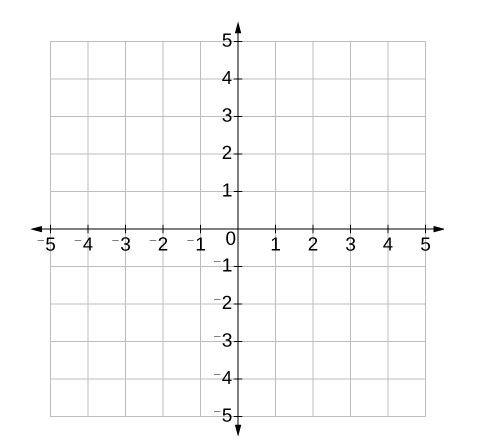
\includegraphics[scale=.75]{../images/cartesian_plane}
\end{figure}

\noindent This plane is also referred to as an "$xy$-plane"; however, the axes are not required to be $x$ and $y$. For example, if we were working on a problem in a physics class, we may refer to the $x$ axis as $t$ (for time) and the $y$ axis as $h$ (for height).

\noindent Positions or placements on the $xy$-plane are referred to as \emph{points} or \emph{ordered-pairs}. All of this together -- the plane, points, axes, etc. -- are collectively referred to as a "\emph{rectangular coordinate system}".

\newpage

\begin{definition}[Point]
written as $(x,y)$ where $x$ is the $x$-coordinate (left/right of the center) and $y$ is the $y$-coordinate (above/below the center)
\end{definition}

\vspace{.15in}

\noindent Regarding individual points, we can make some inferences from our plane.
\begin{itemize}
\item In $Q1$, $x>0$, $y>0$ so our points are $(+,+)$.
\item In $Q2$, $x<0$, $y>0$ so our points are $(-,+)$.
\item In $Q3$, $x<0$, $y<0$ so our points are $(-,-)$.
\item In $Q4$, $x>0$, $y<0$ so our points are $(+,-)$.
\end{itemize}

\vspace{.15in}

\begin{example}
Graph the following points on the coordinate plane below.

\begin{minipage}{.60\textwidth}
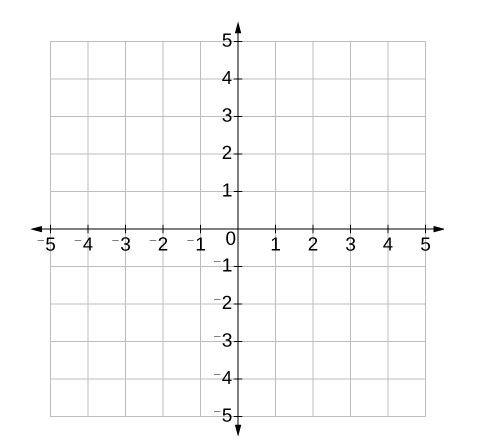
\includegraphics[scale=.75]{../images/cartesian_plane}
\end{minipage}%
\begin{minipage}{.4\textwidth}
\begin{itemize}
\item $A(-2,4)$
\item $B(4,-2)$
\item $C(-3,0)$
\item $D(0,-3)$
\end{itemize}
\end{minipage}%
\end{example}

\newpage

\subsubsection*{Solutions of Equations in 2-Variables}

\noindent A \emph{solution} is an ordered pair $(x,y)$ such that $(x,y)$ satisfies the given equation. Each equation in two variables has an infinite number of solutions -- an infinite number of ordered pairs that satisfy the equation.

\vspace{.15in}

\begin{example}
Is the point $(3,-2)$ a solution to $x-3y=9$?
\vspace{1in}
\end{example}

\begin{example}
Is the point $(-2,3)$ a solution to $x-3y=9$?
\vspace{1in}
\end{example}

\subsubsection*{Finding Solutions}
\begin{enumerate}
\item Choose your $x$ values -- (pick some negative, 0, and some positive)
\item Plug the values of $x$ into the equation and solve for $y$.
\item Write each pair of $x$ and $y$ as an ordered pair.
\end{enumerate}

\vspace{.15in}
\begin{example}
Find 3 solutions of $y=3x+2$.
\end{example}

\newpage

\subsubsection*{Graphing Equations in 2-Variables}
\noindent There are a few methods available to graph these type of equations. The easiest, of course, is to use a graphing calculator. Throughout this chapter we will see a few of the various methods.

\begin{mdframed}
\textbf{Point-Plotting Method}
\begin{enumerate}
\item Find several ordered pairs that are solutions to the equation
\begin{itemize}
\item Aim for 3 or more ordered pairs.
\end{itemize}
\item Plot each of these points on the coordinate plane.
\item Connect the dots - preferably with a straightedge of some sort.
\end{enumerate}
\end{mdframed}

\vspace{.15in}

\begin{example}
Graph the equation $y=3x$.
\vspace{3.5in}
\end{example}

\newpage

\begin{example}
Graph the equation $y=\dfrac{1}{2}x-2$.
\end{example}
\end{document}